\documentclass{beamer}
\usepackage{mathtools}
\usepackage{mathpartir}
\usepackage{semantic}
\usepackage{tikzsymbols}  % This defines \Cat, that we want to redefine
\usepackage{stmaryrd}  % This defines \mapsfrom, that we want to redefine
\usepackage{tikz}
\usetikzlibrary{cd}
\usepackage{adjustbox}
\usepackage{transparent}

\beamertemplatenavigationsymbolsempty
\setbeamertemplate{footline}{
	\raisebox{0.5em}{\makebox[\paperwidth-0.5em][r]{
		\color{gray}\scriptsize\insertframenumber}}}

\input{../../headers/definitions}



\begin{document}
\title {Monoidal Categories and Graphical Calculus}
\author {Felix Rech}
\date {July 19, 2017}

\frame[plain, noframenumbering]{\titlepage}


\begin{frame}[fragile]{Strict Monoidal Category}

  A \demph{strict monoidal category} is a category $C$ with the following:
  \begin{description}[labelindent=foo]
    \item[Tensor product:] A functor $\otimes : C \times C -> C$
    \item[Unit object:] An object $I \in \ob(C)$
    \item[Associativity:] An equality \\
      $(A \otimes B) \otimes C = A \otimes (B \otimes C)$
    \item[Left unit law:] An equality $I \otimes A = A$
    \item[Right unit law:] An equality $A \otimes I = A$
  \end{description}

  \transparent{0}
  Those have to satisfy the \demph{triangle} and \demph{pentagon} equalities:

  \vspace{2ex}

  \begin{adjustbox}{max totalsize={\textwidth}{\textheight}, center}
    \transparent{0}
    \begin{tikzcd}[column sep=0]
      (A \otimes I) \otimes B
        \arrow[dr, "\rho_A \otimes 1_B"']
        \arrow[rr, "\alpha_{A, I, B}"] &&
      A \otimes (I \otimes B)
        \arrow[dl, "1_A \otimes \lambda_B"] \\
      %
      & A \otimes B
    \end{tikzcd}
    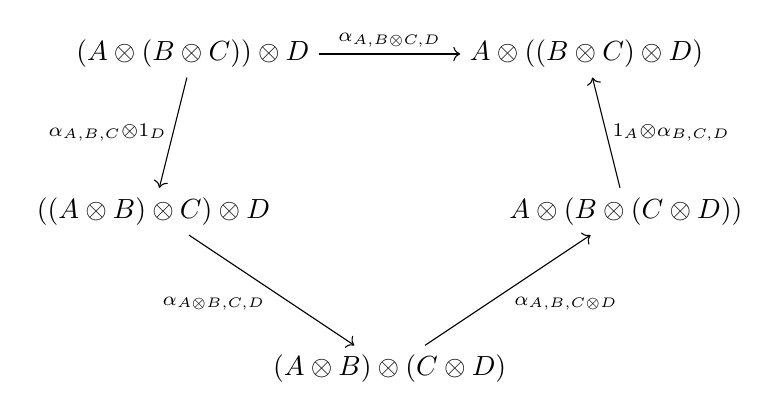
\begin{tikzpicture}[commutative diagrams/every diagram]
      \node (S) at (0, -2)
          {$(A \otimes B) \otimes (C \otimes D)$};
      \node (E) at (3, 0)
          {$A \otimes (B \otimes (C \otimes D))$};
      \node (NE) at (2.5, 2)
          {$A \otimes ((B \otimes C) \otimes D)$};
      \node (NW) at (-2.5, 2)
          {$(A \otimes (B \otimes C)) \otimes D$};
      \node (W) at (-3, 0)
          {$((A \otimes B) \otimes C) \otimes D$};

      \draw[commutative diagrams/.cd, every arrow, every label]
        (NW) edge node[anchor=east] {$\alpha_{A, B, C} \otimes 1_D$} (W)
        (W) edge node[anchor=north east] {$\alpha_{A \otimes B, C, D}$} (S)
        (S) edge node[anchor=north west] {$\alpha_{A, B, C \otimes D}$} (E)
        (E) edge node[anchor=west] {$1_A \otimes \alpha_{B, C, D}$} (NE)
        (NW) edge node {$\alpha_{A, B \otimes C, D}$} (NE);
    \end{tikzpicture}
  \end{adjustbox}

\end{frame}


\begin{frame}[fragile]{Monoidal Category}

  A \demph{monoidal category} is a category $C$ with the following:
  \begin{description}[labelindent=foo]
    \item[Tensor product:] A functor $\otimes : C \times C -> C$
    \item[Unit object:] An object $I \in \ob(C)$
    \item[Associator:] A natural isomorphism \\
      $(A \otimes B) \otimes C \xrightarrow{\smash{\alpha_{A, B, C}}} A \otimes (B \otimes C)$
    \item[Left unitor:] A natural isomorphism $I \otimes A \xrightarrow{\smash{\lambda_A}} A$
    \item[Right unitor:] A natural isomorphism $A \otimes I \xrightarrow{\rho_A} A$
  \end{description}

  \pause
  Those have to satisfy the \demph{triangle} and \demph{pentagon} equalities:

  \vspace{2ex}

  \begin{adjustbox}{max totalsize={\textwidth}{\textheight}, center}
    \transparent{0.6}
    \begin{tikzcd}[column sep=0]
      (A \otimes I) \otimes B
        \arrow[dr, "\rho_A \otimes 1_B"']
        \arrow[rr, "\alpha_{A, I, B}"] &&
      A \otimes (I \otimes B)
        \arrow[dl, "1_A \otimes \lambda_B"] \\
      %
      & A \otimes B
    \end{tikzcd}
    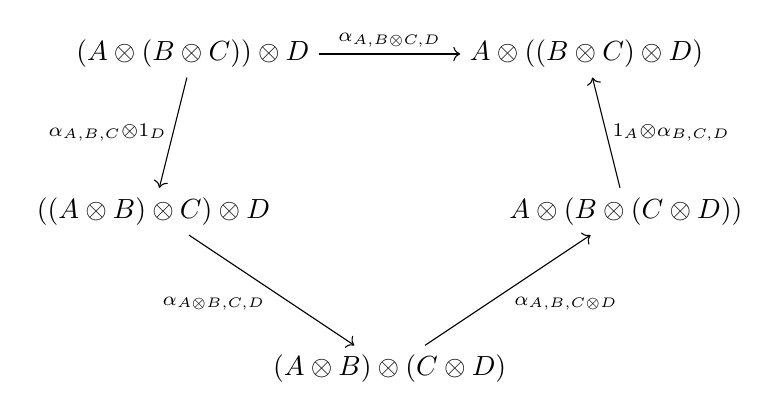
\begin{tikzpicture}[commutative diagrams/every diagram]
      \node (S) at (0, -2)
          {$(A \otimes B) \otimes (C \otimes D)$};
      \node (E) at (3, 0)
          {$A \otimes (B \otimes (C \otimes D))$};
      \node (NE) at (2.5, 2)
          {$A \otimes ((B \otimes C) \otimes D)$};
      \node (NW) at (-2.5, 2)
          {$(A \otimes (B \otimes C)) \otimes D$};
      \node (W) at (-3, 0)
          {$((A \otimes B) \otimes C) \otimes D$};

      \draw[commutative diagrams/.cd, every arrow, every label]
        (NW) edge node[anchor=east] {$\alpha_{A, B, C} \otimes 1_D$} (W)
        (W) edge node[anchor=north east] {$\alpha_{A \otimes B, C, D}$} (S)
        (S) edge node[anchor=north west] {$\alpha_{A, B, C \otimes D}$} (E)
        (E) edge node[anchor=west] {$1_A \otimes \alpha_{B, C, D}$} (NE)
        (NW) edge node {$\alpha_{A, B \otimes C, D}$} (NE);
    \end{tikzpicture}
  \end{adjustbox}

\end{frame}


\begin{frame}

  \begin{theorem}[Coherence for monoidal categories]
    Given the data of a monoidal category, if the pentagon and triangle equations hold, then any well-typed equation built only from $\lambda$, $\rho$ and $\alpha$ and their inverses holds.
  \end{theorem}

\end{frame}


\begin{frame}{Graphical Calculus (1)}

  \begin{definition}
    Two diagrams are \demph{isotopic} when one can be deformed continuously into the other, keeping the boundaries fixed.
  \end{definition}

  \begin{theorem}[Correctness for monoidal categories]
    A well-typed equation between morphisms in a monoidal category follows from the axioms if and only if it holds in the graphical language up to \textbf{planar} isotopy.
  \end{theorem}

  \invisible{
    \begin{theorem}[Correctness for braided monoidal categories]
      A well-typed equation between morphisms in a braided monoidal category follows from the axioms if and only if it holds in the graphical language up to \textbf{spatial} isotopy.
    \end{theorem}

    \begin{theorem}[Correctness for symmetric monoidal categories]
      A well-typed equation between morphisms in a symmetric monoidal category follows from the axioms if and only if it holds in the graphical language up to \textbf{four-dimensional} isotopy.
    \end{theorem}
  }

\end{frame}


\begin{frame}{Braiding}

  A \demph{braided monoidal category} is a monoidal category equipped with a natural isomorphism
  \[ A \otimes B \xrightarrow{\sigma_{A, B}} B \otimes A \]
  satisfying the \demph{hexagon equations}:

  \vspace{2ex}

  \begin{adjustbox}{max totalsize={\textwidth}{\textheight}, center}
    \transparent{0.6}
    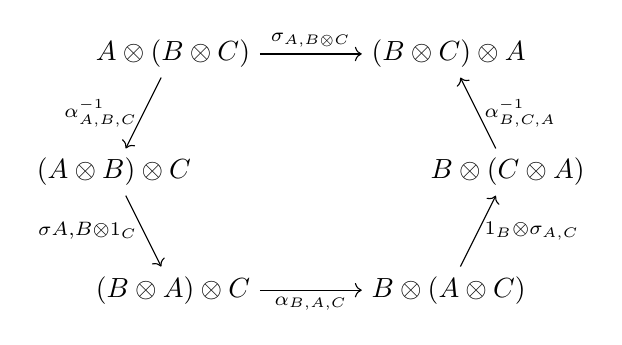
\begin{tikzpicture}[commutative diagrams/every diagram]
      \node (SW) at (-1.75, -1.5)
          {$(B \otimes A) \otimes C$};
      \node (SE) at (1.75, -1.5)
          {$B \otimes (A \otimes C)$};
      \node (E) at (2.5, 0)
          {$B \otimes (C \otimes A)$};
      \node (NE) at (1.75, 1.5)
          {$(B \otimes C) \otimes A$};
      \node (NW) at (-1.75, 1.5)
          {$A \otimes (B \otimes C)$};
      \node (W) at (-2.5, 0)
          {$(A \otimes B) \otimes C$};

      \draw[commutative diagrams/.cd, every arrow, every label]
        (NW) edge node[anchor=east] {$\alpha_{A, B, C}^{-1}$} (W)
        (W) edge node[anchor=east] {$\sigma{A, B} \otimes 1_C$} (SW)
        (SW) edge node[anchor=north] {$\alpha_{B, A, C}$} (SE)
        (SE) edge node[anchor=west] {$1_B \otimes \sigma_{A, C}$} (E)
        (E) edge node[anchor=west] {$\alpha_{B, C, A}^{-1}$} (NE)
        (NW) edge node {$\sigma_{A, B \otimes C}$} (NE);
    \end{tikzpicture}
    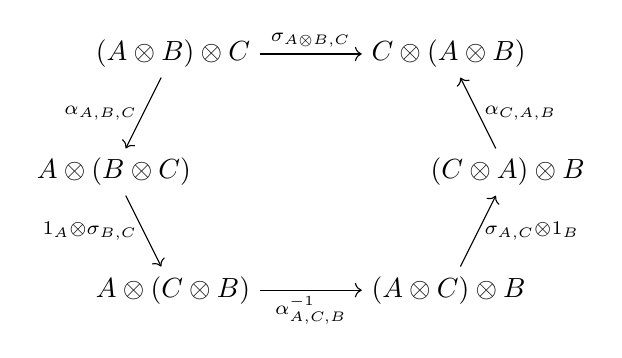
\begin{tikzpicture}[commutative diagrams/every diagram]
      \node (SW) at (-1.75, -1.5)
          {$A \otimes (C \otimes B)$};
      \node (SE) at (1.75, -1.5)
          {$(A \otimes C) \otimes B$};
      \node (E) at (2.5, 0)
          {$(C \otimes A) \otimes B$};
      \node (NE) at (1.75, 1.5)
          {$C \otimes (A \otimes B)$};
      \node (NW) at (-1.75, 1.5)
          {$(A \otimes B) \otimes C$};
      \node (W) at (-2.5, 0)
          {$A \otimes (B \otimes C)$};

      \draw[commutative diagrams/.cd, every arrow, every label]
        (NW) edge node[anchor=east] {$\alpha_{A, B, C}$} (W)
        (W) edge node[anchor=east] {$1_A \otimes \sigma_{B, C}$} (SW)
        (SW) edge node[anchor=north] {$\alpha_{A, C, B}^{-1}$} (SE)
        (SE) edge node[anchor=west] {$\sigma_{A, C} \otimes 1_B$} (E)
        (E) edge node[anchor=west] {$\alpha_{C, A, B}$} (NE)
        (NW) edge node {$\sigma_{A \otimes B, C}$} (NE);
    \end{tikzpicture}
  \end{adjustbox}

  \vspace{2ex}

  \invisible{
    A braided monoidal category is \demph{symmetric} when
    \[ \sigma_{B, A}^{-1} = \sigma_{A, B}. \]
  }

\end{frame}


\begin{frame}{Graphical Calculus (2)}

  \begin{definition}
    Two diagrams are \demph{isotopic} when one can be deformed continuously into the other, keeping the boundaries fixed.
  \end{definition}

  {\transparent{0.2}
    \begin{theorem}[Correctness for monoidal categories]
      A well-typed equation between morphisms in a monoidal category follows from the axioms if and only if it holds in the graphical language up to \textbf{planar} isotopy.
    \end{theorem}
  }

  \begin{theorem}[Correctness for braided monoidal categories]
    A well-typed equation between morphisms in a braided monoidal category follows from the axioms if and only if it holds in the graphical language up to \textbf{spatial} isotopy.
  \end{theorem}

  \invisible{
    \begin{theorem}[Correctness for symmetric monoidal categories]
      A well-typed equation between morphisms in a symmetric monoidal category follows from the axioms if and only if it holds in the graphical language up to \textbf{four-dimensional} isotopy.
    \end{theorem}
  }

\end{frame}


\begin{frame}{Symmetric Braiding}

  A \demph{braided monoidal category} is a monoidal category equipped with a natural isomorphism
  \[ A \otimes B \xrightarrow{\sigma_{A, B}} B \otimes A \]
  satisfying the \demph{hexagon equations}:

  \vspace{2ex}

  \begin{adjustbox}{max totalsize={\textwidth}{\textheight}, center}
    \transparent{0.6}
    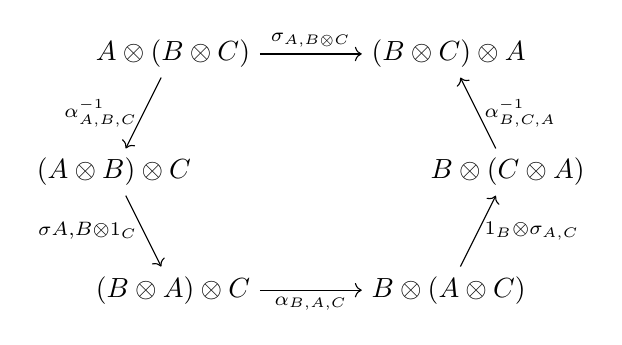
\begin{tikzpicture}[commutative diagrams/every diagram]
      \node (SW) at (-1.75, -1.5)
          {$(B \otimes A) \otimes C$};
      \node (SE) at (1.75, -1.5)
          {$B \otimes (A \otimes C)$};
      \node (E) at (2.5, 0)
          {$B \otimes (C \otimes A)$};
      \node (NE) at (1.75, 1.5)
          {$(B \otimes C) \otimes A$};
      \node (NW) at (-1.75, 1.5)
          {$A \otimes (B \otimes C)$};
      \node (W) at (-2.5, 0)
          {$(A \otimes B) \otimes C$};

      \draw[commutative diagrams/.cd, every arrow, every label]
        (NW) edge node[anchor=east] {$\alpha_{A, B, C}^{-1}$} (W)
        (W) edge node[anchor=east] {$\sigma{A, B} \otimes 1_C$} (SW)
        (SW) edge node[anchor=north] {$\alpha_{B, A, C}$} (SE)
        (SE) edge node[anchor=west] {$1_B \otimes \sigma_{A, C}$} (E)
        (E) edge node[anchor=west] {$\alpha_{B, C, A}^{-1}$} (NE)
        (NW) edge node {$\sigma_{A, B \otimes C}$} (NE);
    \end{tikzpicture}
    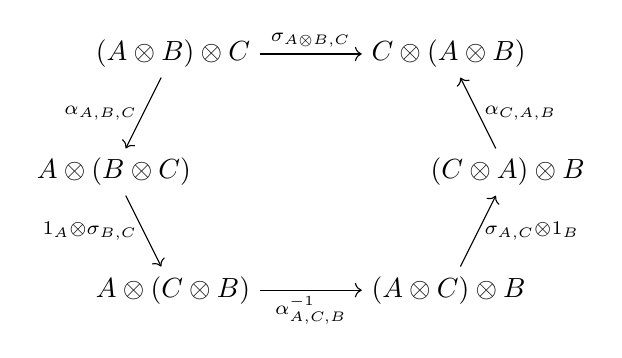
\begin{tikzpicture}[commutative diagrams/every diagram]
      \node (SW) at (-1.75, -1.5)
          {$A \otimes (C \otimes B)$};
      \node (SE) at (1.75, -1.5)
          {$(A \otimes C) \otimes B$};
      \node (E) at (2.5, 0)
          {$(C \otimes A) \otimes B$};
      \node (NE) at (1.75, 1.5)
          {$C \otimes (A \otimes B)$};
      \node (NW) at (-1.75, 1.5)
          {$(A \otimes B) \otimes C$};
      \node (W) at (-2.5, 0)
          {$A \otimes (B \otimes C)$};

      \draw[commutative diagrams/.cd, every arrow, every label]
        (NW) edge node[anchor=east] {$\alpha_{A, B, C}$} (W)
        (W) edge node[anchor=east] {$1_A \otimes \sigma_{B, C}$} (SW)
        (SW) edge node[anchor=north] {$\alpha_{A, C, B}^{-1}$} (SE)
        (SE) edge node[anchor=west] {$\sigma_{A, C} \otimes 1_B$} (E)
        (E) edge node[anchor=west] {$\alpha_{C, A, B}$} (NE)
        (NW) edge node {$\sigma_{A \otimes B, C}$} (NE);
    \end{tikzpicture}
  \end{adjustbox}

  \vspace{2ex}

  A braided monoidal category is \demph{symmetric} when
  \[ \sigma_{B, A}^{-1} = \sigma_{A, B}. \]

\end{frame}


\begin{frame}{Graphical Calculus (3)}

  \begin{definition}
    Two diagrams are \demph{isotopic} when one can be deformed continuously into the other, keeping the boundaries fixed.
  \end{definition}

  {\transparent{0.2}
    \begin{theorem}[Correctness for monoidal categories]
      A well-typed equation between morphisms in a monoidal category follows from the axioms if and only if it holds in the graphical language up to \textbf{planar} isotopy.
    \end{theorem}

    \begin{theorem}[Correctness for braided monoidal categories]
      A well-typed equation between morphisms in a braided monoidal category follows from the axioms if and only if it holds in the graphical language up to \textbf{spatial} isotopy.
    \end{theorem}
  }

  \begin{theorem}[Correctness for symmetric monoidal categories]
    A well-typed equation between morphisms in a symmetric monoidal category follows from the axioms if and only if it holds in the graphical language up to \textbf{four-dimensional} isotopy.
  \end{theorem}

\end{frame}


\begin{frame}[t, fragile]{Dual Objects}

  In a monoidal category, an object $L$ is \demph{left-dual} to an object $R$, and $R$ is \demph{right-dual} to $L$, written $L \dashv R$, when there exist
  \begin{itemize}
    \item a \demph{unit} morphism $I \xrightarrow{\eta} R \otimes L$ and
    \item a \demph{counit} morphism $L \otimes R \xrightarrow{\varepsilon} I$
  \end{itemize}
  satisfying the \demph{snake equations}:

  \vspace{2ex}

  \begin{adjustbox}{max width=\linewidth, center}
  \transparent{0.6}
  \begin{tikzcd}
    L \arrow[r, "\rho_L^{-1}"] \arrow[d, "1_L"] &
    L \otimes I \arrow[r, "1_L \otimes \eta"] &
    L \otimes (R \otimes L) \arrow[d, "\alpha_{L, R, L}^{-1}"] \\
    %
    L &
    I \otimes L \arrow[l, "\lambda_L"] &
    (L \otimes R) \otimes L \arrow[l, "\varepsilon \otimes 1_L"]
  \end{tikzcd}
  \begin{tikzcd}
    R \arrow[r, "\lambda_R^{-1}"] \arrow[d, "1_R"] &
    I \otimes R \arrow[r, "\eta \otimes 1_R"] &
    (R \otimes L) \otimes R \arrow[d, "\alpha_{R, L, R}"] \\
    %
    R &
    R \otimes I \arrow[l, "\rho_R"] &
    R \otimes (L \otimes R) \arrow[l, "1_R \otimes \varepsilon"]
  \end{tikzcd}
  \end{adjustbox}

\end{frame}


\begin{frame}[t]{Properties of Duals}

  \begin{lemma}
    The left- and right-dual of an object are unique.
  \end{lemma}

  \pause

  \begin{lemma}
    The unit of a duality determines the counit and vice-versa.
  \end{lemma}

  \pause

  \begin{lemma}
    In a monoidal category $I \dashv I$.
  \end{lemma}

  \pause

  \begin{lemma}
    In a monoidal category $L \dashv R$ and $L' \dashv R'$ implies $L \otimes L' \dashv R' \otimes R$.
  \end{lemma}

  \pause

  \begin{lemma}
    In a braided monoidal category $L \dashv R$ implies $R \dashv L$.
  \end{lemma}

\end{frame}


\end{document}
